% mnras_template.tex 
%
% LaTeX template for creating an MNRAS paper
%
% v3.0 released 14 May 2015
% (version numbers match those of mnras.cls)
%
% Copyright (C) Royal Astronomical Society 2015
% Authors:
% Keith T. Smith (Royal Astronomical Society)

% Change log
%
% v3.0 May 2015
%    Renamed to match the new package name
%    Version number matches mnras.cls
%    A few minor tweaks to wording
% v1.0 September 2013
%    Beta testing only - never publicly released
%    First version: a simple (ish) template for creating an MNRAS paper

%%%%%%%%%%%%%%%%%%%%%%%%%%%%%%%%%%%%%%%%%%%%%%%%%%
% Basic setup. Most papers should leave these options alone.
\documentclass[letters,usenatbib,times]{mnras}

% MNRAS is set in Times font. If you don't have this installed (most LaTeX
% installations will be fine) or prefer the old Computer Modern fonts, comment
% out the following line
\usepackage{newtxtext,newtxmath}
% Depending on your LaTeX fonts installation, you might get better results with one of these:
%\usepackage{mathptmx}
%\usepackage{txfonts}

% Use vector fonts, so it zooms properly in on-screen viewing software
% Don't change these lines unless you know what you are doing
\usepackage[T1]{fontenc}

% Allow "Thomas van Noord" and "Simon de Laguarde" and alike to be sorted by "N" and "L" etc. in the bibliography.
% Write the name in the bibliography as "\VAN{Noord}{Van}{van} Noord, Thomas"
\DeclareRobustCommand{\VAN}[3]{#2}
\let\VANthebibliography\thebibliography
\def\thebibliography{\DeclareRobustCommand{\VAN}[3]{##3}\VANthebibliography}


%%%%% AUTHORS - PLACE YOUR OWN PACKAGES HERE %%%%%

% Only include extra packages if you really need them. Common packages are:
\usepackage{graphicx}	% Including figure files
%% \usepackage{amsmath}	% Advanced maths commands
%% \usepackage{amssymb}	% Extra maths symbols

%%%%%%%%%%%%%%%%%%%%%%%%%%%%%%%%%%%%%%%%%%%%%%%%%%

%%%%% AUTHORS - PLACE YOUR OWN COMMANDS HERE %%%%%

% Please keep new commands to a minimum, and use \newcommand not \def to avoid
% overwriting existing commands. Example:
%\newcommand{\pcm}{\,cm$^{-2}$}	% per cm-squared

%%%%%%%%%%%%%%%%%%%%%%%%%%%%%%%%%%%%%%%%%%%%%%%%%%

%%%%%%%%%%%%%%%%%%% TITLE PAGE %%%%%%%%%%%%%%%%%%%

% Title of the paper, and the short title which is used in the headers.
% Keep the title short and informative.

\title[High-resolution ALMA observations of V4046\,Sgr]{High-resolution ALMA observations of V4046\,Sgr: a circumbinary disc with a thin ring}

% The list of authors, and the short list which is used in the headers.
% If you need two or more lines of authors, add an extra line using \newauthor
\author[R. Martinez Brunner et al.]{
Rafael Martinez-Brunner,$^{1}$\thanks{E-mail: rmartinezbrunner@gmail.com}
Simon Casassus,$^{1}$
Sebasti\'an P\'erez,$^{2}$
et al. 
\\
% List of institutions
$^{1}$Departamento de Astronom\'{\i}a, Universidad de Chile, Casilla 36-D, Santiago, Chile\\
$^{2}$Universidad de Santiago de Chile, Av. Ecuador 3659, Santiago\\
}

% These dates will be filled out by the publisher
\date{Accepted XXX. Received YYY; in original form ZZZ}

% Enter the current year, for the copyright statements etc.
\pubyear{2020}

% Don't change these lines
\begin{document}
\label{firstpage}
\pagerange{\pageref{firstpage}--\pageref{lastpage}}
\maketitle

% Abstract of the paper
\begin{abstract}
  The nearby V4046\,Sgr spectroscopic binary  hosts a gas-rich disc known for its wide cavity and dusty ring. We present new high resolution ($\sim$20\, mas) ALMA observations of the 1.3\,mm  continuum. The comparison of these  observations, combined with SPHERE-IRDIS polarized  images and a well-sampled spectral energy distribution (SED), against radiative transfer (RT) predictions carried out with the RADMC3D package, allow us to propose a physical model for the source. The new ALMA data reveal a very fine ring at a radius of 13.46$\pm$0.43\,au (Ring13), with a marginally resolved radial width of  4.17$\pm$0.94\,au.  Ring13 is the brightest structure in scattered-light, where it is surrounded by a $\sim$9\,au-wide gap , and it is flanked by a very bright mm outer ring (Ring24) with a sharp inner edge at 24\,au. The steeply decreasing radial slope of Ring24 breaks at $\sim$35\,au into a shallow tail. The RT model requires an inner ring at $\sim$6\,au (Ring6) in small dust grains, hiding under the IRDIS coronagraph, and that surrounds an inner circumbinary disk. Faint mm-continuum coincident with Ring6 is picked up by ALMA, whose morphology  suggests that Ring6  is lopsided or shadowed by the secondary. The previously reported scattered-light shadow of the secondary star is  also reproduced by the RT model.  The surpising  thin Ring13 is nonetheless **10*** times wider than the model scale height, and could thus be long-lived.   The strong near-far disc asymmetry  at 1.65\,$\micron$ points at a very forward-scattering phase function, and requires  grain radii  of no less than  0.4\,$\micron$. 
\end{abstract}

% Select between one and six entries from the list of approved keywords.
% Don't make up new ones.
\begin{keywords}
 protoplanetary discs -- submillimetre: planetary systems -- radiative transfer
\end{keywords}

%%%%%%%%%%%%%%%%%%%%%%%%%%%%%%%%%%%%%%%%%%%%%%%%%%

%%%%%%%%%%%%%%%%% BODY OF PAPER %%%%%%%%%%%%%%%%%%


\section{Introduction} \label{sec:Introduction}

Recent observations of young circumstellar discs have transformed  current knowledge of planet formation, but the focus of resolved imaging with the Atacama Large Millimeter/submillimetre Array (ALMA) or with VLT/SPHERE has  mainly been towards the brighter sources \citep[see][for a review]{Andrews2020arXiv200105007A}. The Disks ARound T Tauri Stars (DARTTS) program was first presented in \citet{Avenhaus_2018} with the aim to image eight stars with the Spectro-Polarimeter High-contrast Exoplanet REsearch (SPHERE). The sample is not biased towards exceptionally bright and large disks, and consists of only solar-mass stars. A second part of the survey increased the number of sources by presenting 21 new images of circumstellar disks \citep{Garufi2020}. The observations revealed diversed structures and morphologies in the scattering surface of these disks. This letter on V4046 Sagittarii (Sgr) is part of our new DARTTS survey with ALMA (DARTTS-A) which will present millimeter observations of nine protoplanetary disks previously imaged in polarized scattered light in DARTTS-S.  



V4046\,Sgr is a double-lined spectroscopic binary of K-type stars (K5 and K7) with very similar masses of 0.90$\pm$0.05\,M$_{\sun}$ and 0.85$\pm$0.04\,M$_{\sun}$ \citep{Rosenfeld_2012} on a close ($a \approx 0.041$\,au), circular ($e\leq0.001$) orbit, with an orbital period of 2.42 days \citep{refId0}. It is a member of the $\beta$ Pictoris moving group \citep{Zuckerman_2004}, with an estimated age of 23$\pm$3\,Myr \citep{Mamajek_2014}, and its distance is  72.41$\pm$0.34\,pc \citep{Gaia}. V4046\,Sgr hosts a massive ($\sim$0.1\,M$_{\sun}$) circumbinary disc extending to $\sim$300\,au \citep{Rosenfeld_2013, Rodriguez_2010}, with a rich observable chemical  diversity  \citep{Kastner_2018}. 


The structure of this letter is as follows. The observations, including  new 1.3\,mm continuum data, are described in Section \ref{sec:Observations}. We interpret the data in terms of a parametric model,  presented in Section \ref{sec:model}. Previous models of V4046\,Sgr have been made \citep{Ru_z_Rodr_guez_2019, Rosenfeld_2013, 2019ApJ...882..160Q} but our new ALMA data bring additional information. Our results are discussed in  Section \ref{sec:results} and summarised in  Section \ref{sec:Conclusions}.

\section{Observations} \label{sec:Observations}

%% Disc structures can be explored by means of comparing mm continuum and scattered-light images. These observations allow us to see the distribution of different populations of dust particles, while ALMA traces the millimetre-sized grains settled in the mid-plane of the disc, scattered-light imaging accounts for photons reflected off small micron-sized dust at the disc surface layer, high above the mid-plane. By comparing both, is easier to determine whether asymmetries in scattered light correspond to surface ripples or deep structures intrinsic to the underlying density distribution. 

New ALMA observations of V4046\,Sgr were obtained in 2017 as part of the Cycle 5 program 2017.1.01167.S (PI: S. Perez). These were acquired in the context of the DARTTS-A program (Perez et al. {\em in prep}), a larger survey for 9 optically visible TTauri discs at $\sim$50\,mas resolution. The survey simultaneously mapped the 1.3\,mm continuum and the J = 2$-$1 line of $^{12}$CO with the C43-8 array configuration in band 6 (211-275\,GHz). This work focuses exclusively on the data obtained in the 1.3\,mm continuum for our source, taken with a beam size of $0\farcs04 \,\times \, 0\farcs06$ (in natural weights). **Seba, sure that the survey only used C43-8?***

In this investigation, we use the  polarimetric image at 1.65\,$\micron$ previously published as part of the DARTTS-SPHERE I survey \citep{Avenhaus_2018}. The image was taken at the ESO Very Large Telescope with the SPHERE-IRDIS instrument in differential polarization imaging (DPI) mode, and a complete description of the data reduction was presented in \citet{Avenhaus_2018}. 

For our analysis of the ALMA image we used an image reconstruction strategy, using the non-parametric image synthesis of the \textsc{uvmem} package \citep{2006ApJ...639..951C, 2018A&C....22...16C} it is possible to super-resolve the clean beam, obtaining an effective angular resolution $\sim$3 times finer than  natural weights. The model image is obtained by fitting the data using Chi-squared minimisation, with a measure of regularization when required. Here we adopted a pure $\chi^2$ model image ***sure about this? what is the name of the image you used?****. The resulting \textsc{uvmem} image shown in Fig. \ref{fig:two} exhibits previously unseen substructure of the disc. This image reveals that the disc features two rings of large dust grains with a broad gap between them, i.e. Ring13  at 13\,au and Ring24 starting at 24\,au. The wide and bright  Ring24  reaches its peak intensity at $\sim$30\,au, beyond which it drops steeply before breaking at  $\sim$35\,au into a  shallow tail. While this is the first observation of Ring13,  \citet{Ru_z_Rodr_guez_2019} did anticipate its existence ****HOW? EXPAND ON THIS***

\begin{figure*}
  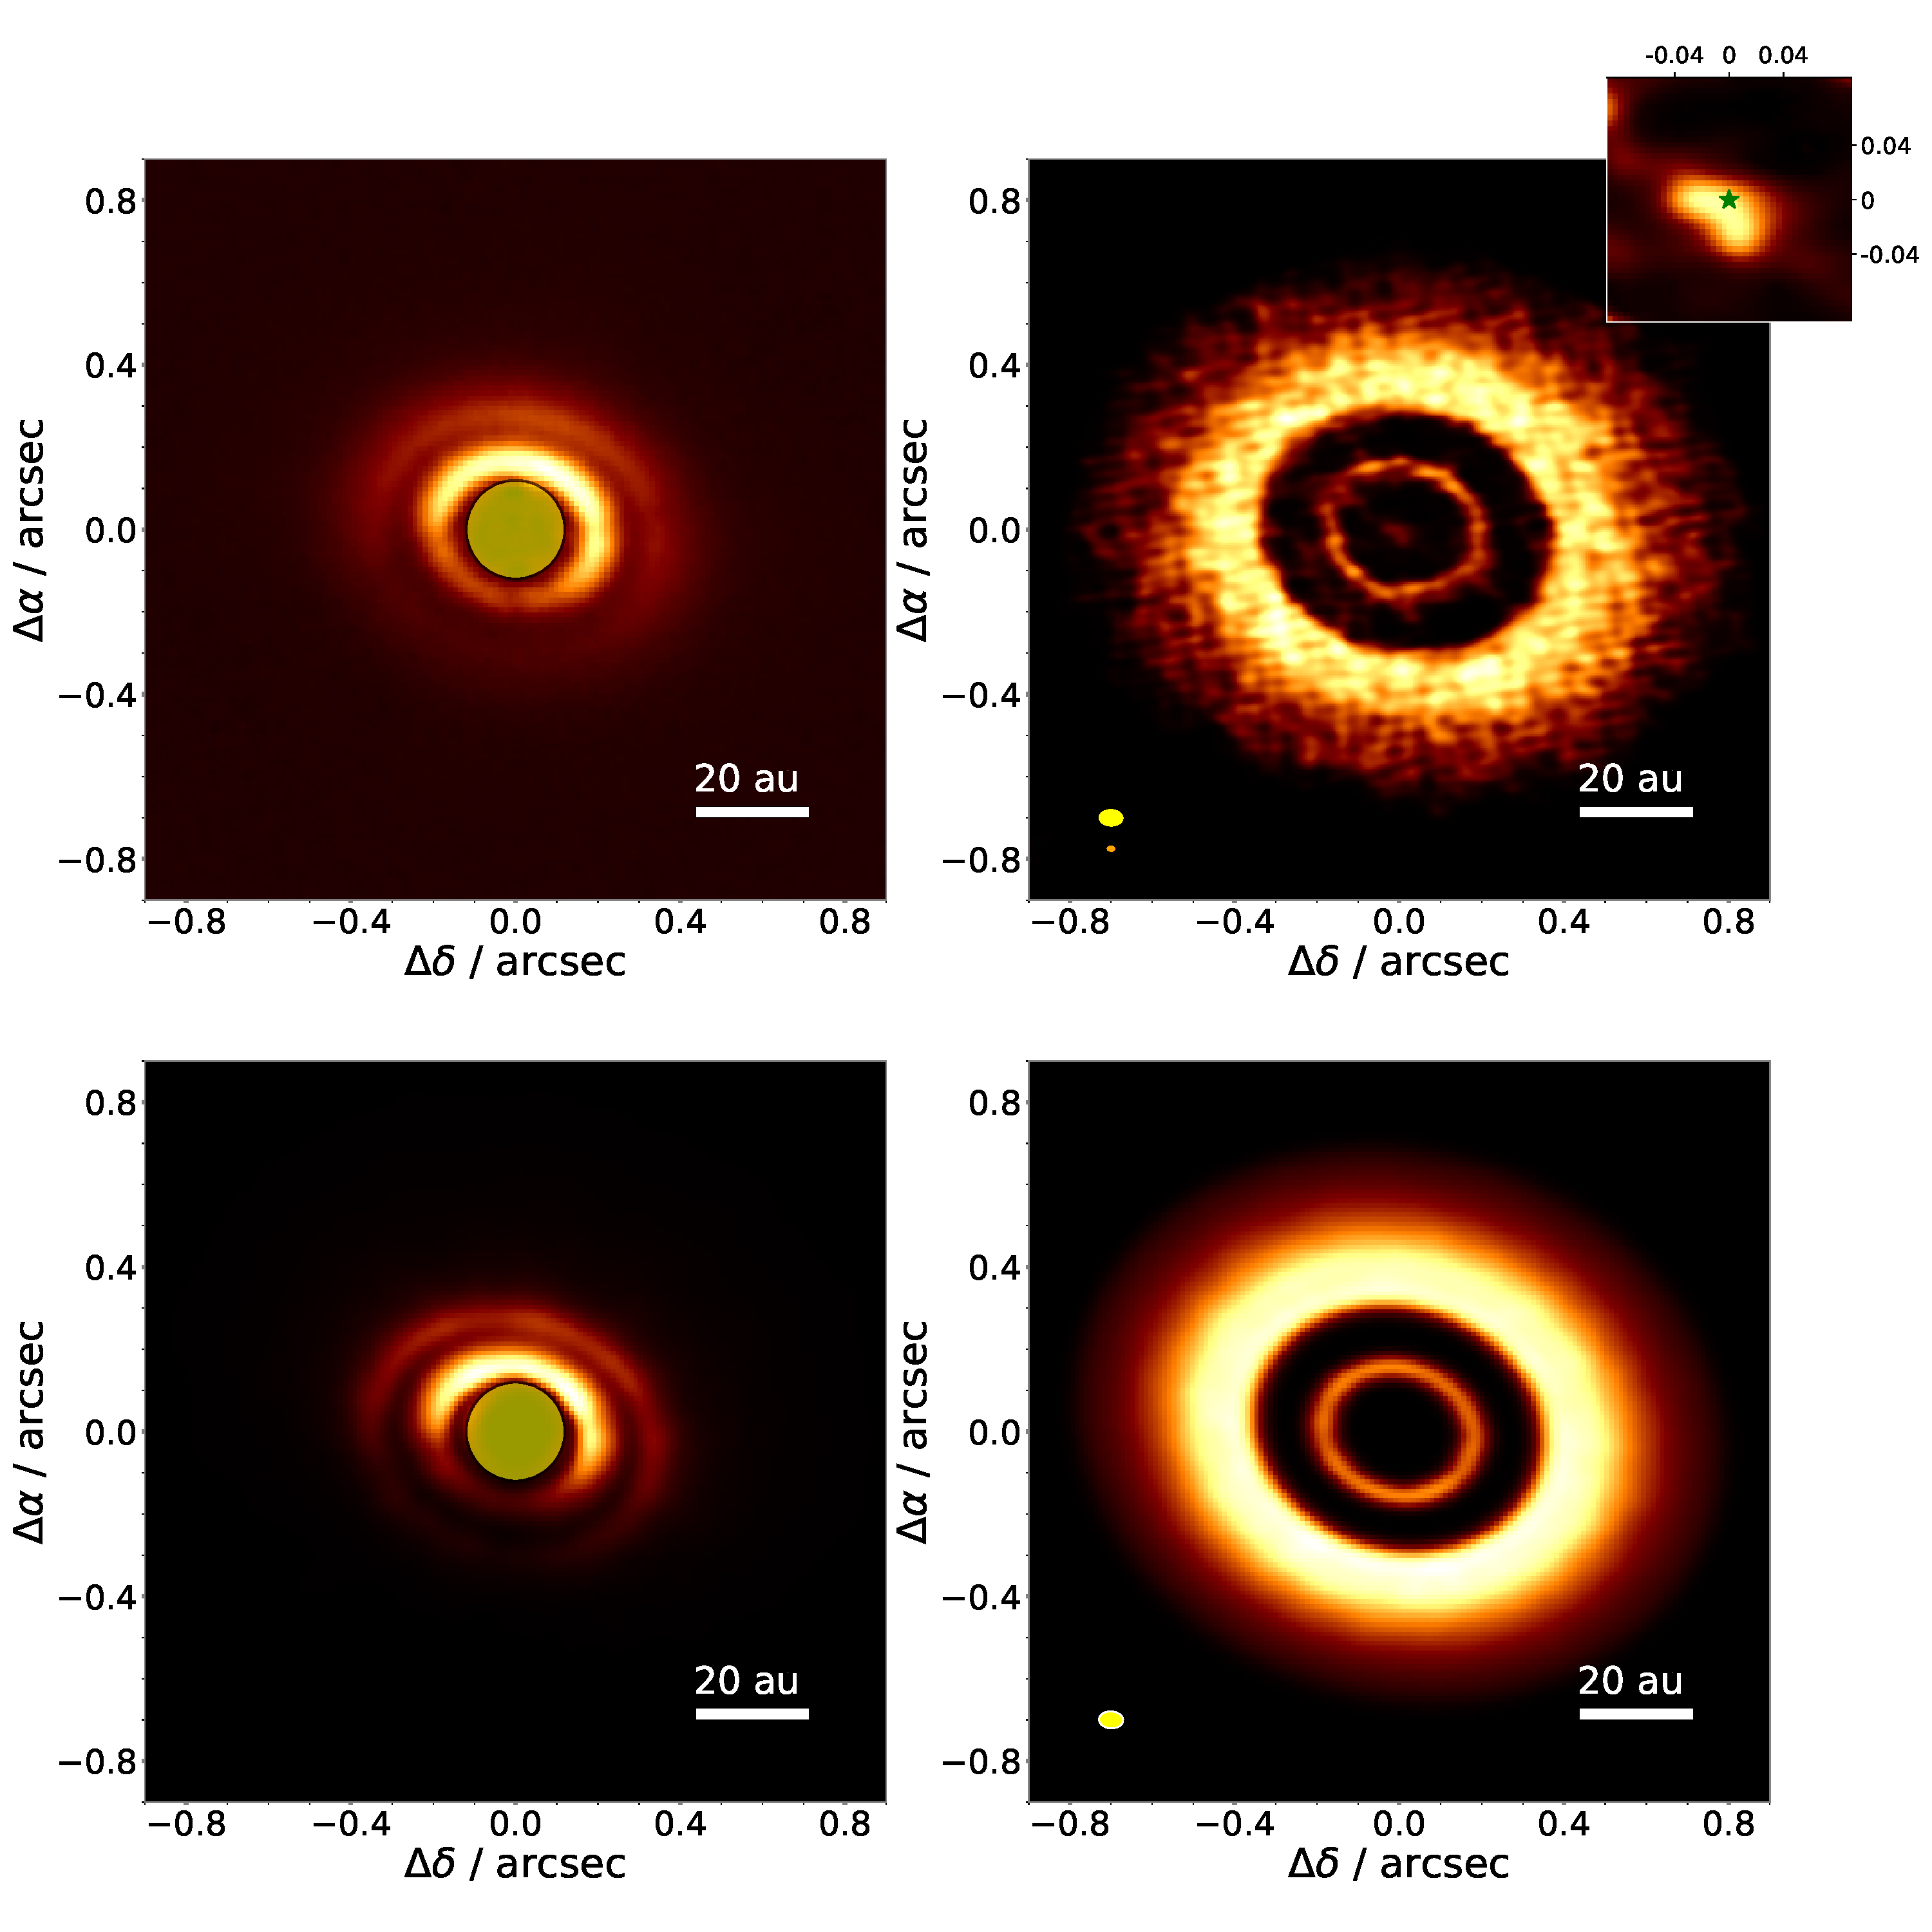
\includegraphics[width=\textwidth]{hot_two_E.pdf}
  \caption{Comparison of observations and simulated images at 1.65\,$\micron$ and 1.3 mm continuum of the circumbinary disc orbiting V4046\,Sgr. From top to bottom: DPI image and ALMA Band 6 observations; simulated images of the parametric model. Top left panel: SPHERE-IRDIS \textit{H}-band image with a yellow filled circle that illustrate the N\_ALC\_YJH\_S coronagraph (inner working angle $\sim0\farcs12$, or $\sim$8.6\,au at 72.4\,pc). Top right panel: 1.3\,mm continuum \textsc{uvmem} model image. The yellow ellipse shows the size of the natural-weighted beam: $ 0\farcs04 \, \times \, 0\farcs06$. The inset zooms into  the central emission, and the green star marks the star positions. Bottom left panel: 1.65\,$\upmu m$ simulated image of the parametric model. Bottom right panel: 1.3\,mm simulated image of the parametric model. The yellow ellipse shows the size of the  beam: $ 0\farcs04 \, \times \, 0\farcs06$ ***ESTOY CONFUNDIDO POR ESTE BEAM, HAY QUE REPORTAR  1/3 BMAJxBMIN / BPA, INDICANDO 1/3 SEGUIDO POR LOS VALORES EN PESOS NATURALES, Y PLOTEAR EL RESULTADO *****. For all the images in the figure the colour scale is linear.}
  \label{fig:two}
\end{figure*}

Ring13 is surprisingly narrow and seems to be off-centre relative to the GAIA stellar position (at the origin of coordinates in Fig. \ref{fig:two}). We determined the ring's center and orientation by  minimising  the dispersion of the disc radial profiles, from 6\,au to 19\,au, and thus obtained a  PA of 74.6\,$\degr$ ***ADD ERRORES***, an inclination of 33.9\,$\degr$ **ERRORS**** and a centre at $\Delta \alpha = 9\pm0.05$\,mas $\Delta \delta = 0.1\pm0.04$\,mas, relative to the stars.

The ring width can be measured in polar coordinates by fitting 1-D Gaussians, thus  obtaining a width and centroid at each azimuth. On average, we obtained  a FWHM of 4.17$\pm$0.94\,au, and a stellocentric radius of  13.46$\pm$0.43\,au  (See Fig. \ref{fig:polarring}). As the \textsc{uvmem} model image has an effective angular resolution of $\sim$1/3 that of the natural-weighted beam ($0\farcs04 \,\times \, 0\farcs06$) ***CREO QUE AHORA ENTIENDO, HAY QUE ASEGURARTE QUE ESTOS SON LOS BEAMS - DEBIERA SER BMAJORxBMINOR. NO CALZA CON EL ABSTRACT ESO SI***, we see that Ring13 is marginally resolved. After subtaction of the approximate {\tt uvmem} resolution, the ring width is $\sim$*****. 
****SUBTRACT UVMEM BEAM IN QUADRATURE.****


Repeating the optimization of the disk orientation, but  this time aiming for Ring24  with a radiual domain from 20\,au to 70\,au, we obtained a  PA of 76.8\,$\degr$ ***ERROrSS***, with an inclination of 34.0\,$\degr$ **ERRORS* and a centre at $\Delta \alpha = 19\pm0.04$\,mas $\Delta \delta = 7\pm0.03$\,mas relative to the stars. We see that both Ring13 and Ring24  both share / DO NOT SHARE? the same orientation and center, given the errors, and both are offset from the star. Even though all orientation parameters for Ring13 and Ring24  are consistent within the errors, there  are however some hints for a different orientation, as summarised in Fig. \ref{fig:polarring}, perhaps due to the joint effect of all these small differences. ****CALCULATE THE CHI2 DIFFERNCE BETWEEN THE TWO TRACES? SOME FORM OF STATS WOULD BE GOOD**** 


***I WOULD REMOVE THIS OR IDENTIFY SOMETHING CONCRETE OUT OF IT: We can compare the measured location of the inner ring according to  these parameters versus to the location obtained before. The deviation for each azimuth is shown in Fig. \ref{fig:polarring}, and is not trivial since it depend on a few parameters such as the different inclinations of the rings, the difference in position angle and the shift of the centres relative to the stars. But even though those parameters play an important role, a possible small difference in eccentricities between the inner and the outer ring could also help explain this deviation between the two measurements. ***



Interestingly, the ALMA image also detects faint 1.3\,mm continuum emission near the stellar positions (See the inset in Fig. \ref{fig:two}). Since this faint central emission is offset from the star, at the origin of coordinates in the figure, it is probably due to large dust grains. This dust structure is at a distance of only $\sim0\farcs02$ from the binary system.

The scattered-light image shown in Fig. \ref{fig:two} also shows  a double ring structure in the micron-sized dust distribution. The observed morphology presents an inner cavity of $\sim$10\,au in radius and two rings located at 14.10$\pm$0.01, coincident with Ring13,  and 24.62$\pm$0.08\,au, coincident with Ring24,  with a small gap between them at $\sim$20\,au. The observed second ring  matches   the inner wall of the 1.3\,mm continuum emission outer ring \citep{Ru_z_Rodr_guez_2019}. Two other important features that are present in the image are: the brightness asymmetry and the shadows projected on the disc produced by the close binary system as they eclipse each other, described in detail by \citet{dOrazi}.


\citet{dOrazi} reported a  binary phase in the scattered-light observation around 106\,$\degr$, setting $\phi=$0 from the North and increasing clockwise. Using this measurement, the binary phase was calculated at the time of the ALMA observation at $\phi=$13\,$\degr$. There is no clear signal of any shadow similar to the ones present in the DPI image, this could be explained by innefficient disk cooling compared to the speed of the illumination pattern \citep[][]{Casassus2019MNRAS.486L..58C} ***NO ERA DIFICIL ENCONTRAR ESA REF, PORFA LEER AL MENOS EL ABSTRACT****


\begin{figure}
    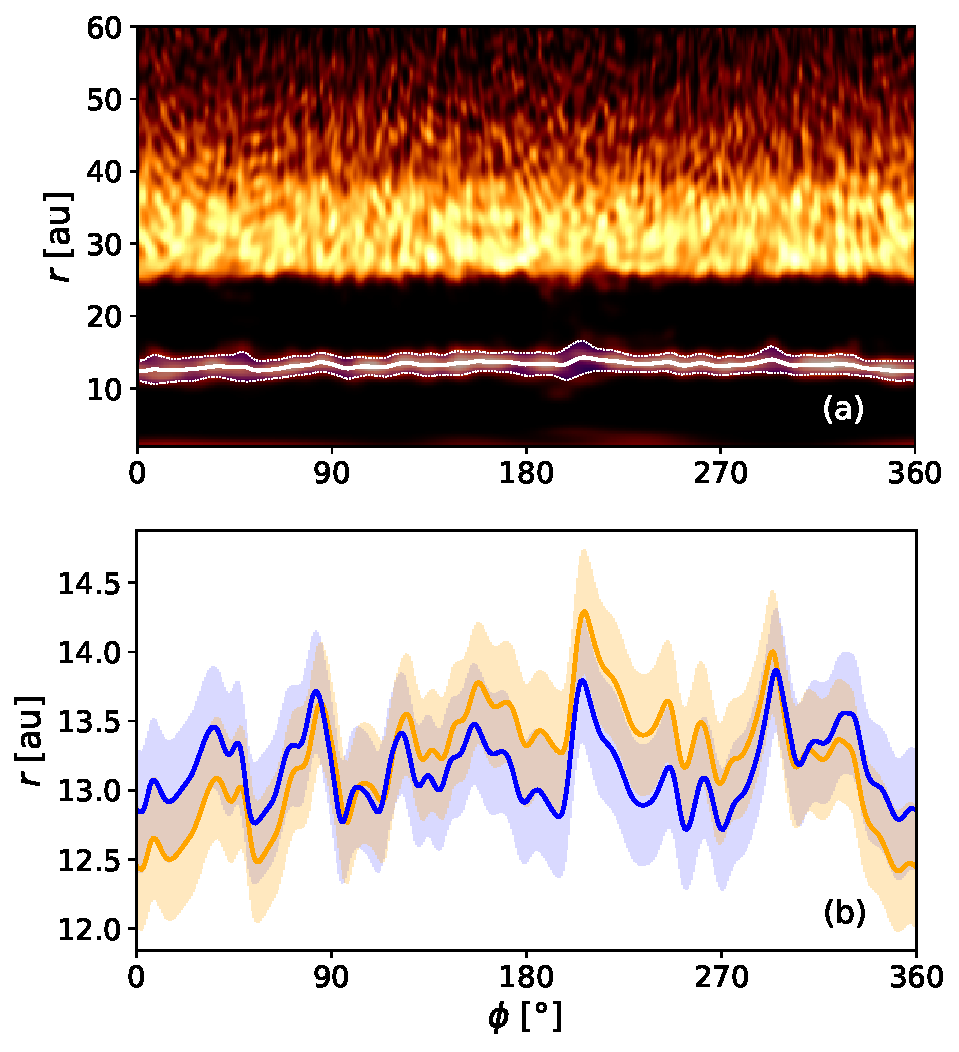
\includegraphics[width=\columnwidth]{polar_ring_aprox_and_diff_inner.pdf}
    \caption{(a) Polar decomposition of the 1.3\,mm continuum image, using the orientation of Ring24. We  trace Ring13 using the centroids  (solid line) and width of radial Gaussian fits  (blue region between the dotted lines). (b) Centroid of Ring13, for two disc orientations: the orange line corresponds to the same trace as in a), while the  blue line is  obtained for the inner ring orientation.}
    \label{fig:polarring}
\end{figure}

\begin{figure}
	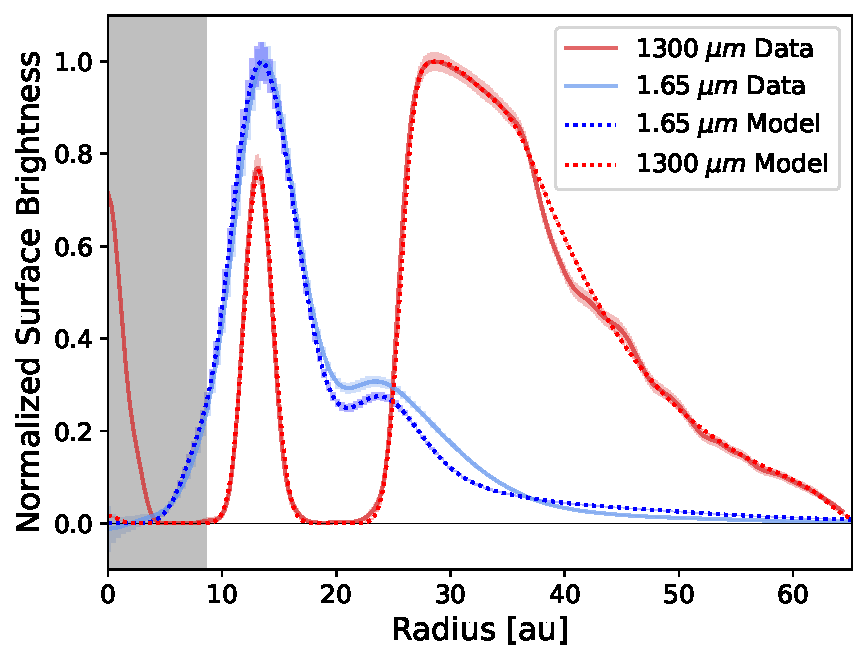
\includegraphics[width=\columnwidth]{comp_fig_all_profiles_au.pdf}
    \caption{Comparison of the surface brightness profiles extracted from the deprojected synthetic images and observed \textit{H}-band and 1.3\,mm continuum images. The grey shaded area represents the inner working angle of the artificial coronagraph used in the simulations (i.e., $\sim0\farcs 12$, or $\sim$8.6\,au at 72.4\,pc).}
    \label{fig:radprofiles}
\end{figure}



***HASTA AQUI LLEGUE*****
\section{Parametric radiative transfer model} \label{sec:model}

To search for a possible model that could explain the available data, we perform radiative transfer modelling with \textsc{radmc3d} \citep{Dullemond_2012}. Here we describe a 3D modelling framework for constructing disc structures given some parameters to characterise it. The model environment is similar to the one used by \citet{2018MNRAS.477.5104C} for DoAr 44. Through trial and error, we look for a set of values for the parameters that can define a model that correctly fits the available data.

For the representation of the stars, we used two Kurucz photospheres models \citep{1979ApJS...40....1K, 1997A&A...318..841C} with T$_{\mathrm{eff},1} =$ 4350\,K, R$_{*,1} =$ 1.064\,R$_{\sun}$, M$_{*,1} =$ 0.90\,M$_{\sun}$ and T$_{\mathrm{eff},2} =$ 4060\,K, R$_{*,2} =$ 1.033\,R$_{\sun}$, M$_{*,2} =$ 0.85\,M$_{\sun}$ respectively and with an accretion rate of log$\,\dot{\mathrm{M}} = -$9.3\,Myr$^{-1}$ for both cases \citep{10.1111/j.1365-2966.2011.19366.x}. The stars were placed with a separation of 0.041\,au and oriented with a 30\,$\degr$ rotation, relative to the semi-major axis of the disk, to match the shadows reported by \citet{dOrazi}.

Recreating the complex radial and vertical structure of the V4046\,Sgr disc is not an easy task. We choose to build the model by thinking the components of the disc separately and then unite them as a whole. Given the observations that we are using, we consider that a correct approach for this disc is using two different dust populations: larger grains that are vertically settled and dominates the disc mass and a less-abundant population of smaller grains that are distributed to larger heights from the mid-plane. As the gas and the small-dust population are coupled, it is important to consider the gas in the modelling process, but no line emission prediction is made. 

Assuming a three dimensional model in a spherical reference frame with coordinates ($r$, $\theta$, $\phi$), the gas density ($\rho_{\mathrm{gas}}$) distribution follows
\begin{equation}
  \rho_{\mathrm{gas}}(r,z) =\frac{\Sigma(r) \,\delta(r)}{\sqrt{2\pi} \,r H(r)}  \mathrm{exp}\left[-\frac{1}{2} \left(\frac{z}{r H(r)}\right)^2\right].
\end{equation}
Where $\delta(r)$ is a parameter that indicates the density drops in the gaps and cavities, $H(r)$ is the scale height profile and $\Sigma(r)$ been the surface density profile. $\Sigma(r)$ is defined by
\begin{equation}
  \Sigma(r) = \Sigma_\mathrm{c} \left(\frac{r}{R_\mathrm{c}}\right)^{-\gamma}  \, \mathrm{exp}\left[-\left(\frac{r}{R_\mathrm{c}}\right)^{2-\gamma}\right],
\end{equation}
where $R_c$ is a characteristic radius and $\gamma$ is the surface density gradient. A fixed $\gamma$ = 1 is used as it is a typical value for discs \citep{Andrews_2009,Andrews_2010}. 

We define the parametric scale height profiles for the gas and for each dust population as
\begin{equation}
    \label{scale}
  H(r)=\chi \, H_{o}(r) \, [r/r_{o}(r)]^{\psi(r)},
\end{equation}
where $H_o$ is the scale height at r = $r_o$, $\psi$ is the flaring index and $\chi$ is a scaling factor (in the range $0-1$) that mimics dust settling. For the gas and the micron-sized grains $\chi$ = 1 and for the millimetre-size dust population, as \citet{Rosenfeld_2013}, we assign a fixed $\chi$ = 1/2 for simplicity.

The small-dust density distribution follows the same behaviour as the gas but with different scaling factors: the dust-to-gas ratio ($\zeta$ = 0.047 as \citet{Rosenfeld_2013}), the mass fraction between small and large dust particles ($f_{\mathrm{mass}}$) and another $\delta_{\mathrm{sd}}(r)$ factor for fine tuning that depends on the radius. So it is
\begin{equation}
\rho_{\mathrm{small-dust}}(r,z)=\rho_{\mathrm{gas}}(r,z)\, f_{\mathrm{mass}} \, \delta_{\mathrm{sd}}(r) \: \zeta .
\end{equation}

Since the large-dust grains are less coupled to the gas, their distribution has some important differences. A large inner cavity and another scaling factor (or filter) is needed to generate the larger gap between the rings. For the inner ring, the same profile as the gas is used, but with different values for $R_c$ and $\Sigma_c$. The greatest difference is in the outer ring, where we used a sum of an exponential correction with a Gaussian function and, between 32 and 34.5\,au, in an effort to recreate the break seen in the profile, we chose a different value for $\gamma$ = -8. So, for the large dust grains, the surface density is 

\begin{multline}
  \Sigma_{\mathrm{large-dust}}(r) = \Sigma_{\mathrm{c}2} \left(\frac{r}{R_{\mathrm{c}2}}\right)^{-\gamma}  \\ \, \left\{ \mathrm{exp}\left[-\left(\frac{r}{R_{\mathrm{c}2}}\right)^{2-\gamma}\right] +  \mathrm{exp}\left[-\left(\frac{r}{R_{\mathrm{c}2}}\right)^{2}\right]\right\}.
\end{multline}

Also for both dust populations, the inner part of the outer ring follows a different behaviour. The surface density profile is multiplied by an additional factor
\begin{equation}
    \epsilon(r) = \delta +  (1 - \delta) \left(\frac{ r - R_\mathrm{in}}{R_\mathrm{peak} - R_\mathrm{in}}\right)^3,
\end{equation}
where $\delta=10^{-4}$ and $R_\mathrm{in}$ and $R_\mathrm{peak}$ would depend on the dust population, marking the beginning and the maximum density peak of the outer ring. This parameter allow us to model a smoother inner wall of the outer ring.

The two different populations of dust grains vary in size, the small grains range from  0.4 to 1.5\,$\micron$ and the large dust grains range from 0.4\,$\micron$ to 10\,mm. For absorption and opacities of dust populations we assume a typical ISM mineralogical composition, containing 70\% silicate and 30\% graphite.

In an effort to obtain a similar asymmetry as the one observed in the DPI image, the simulated image at 1.65\,$\micron$ had to be taken using a special grain size distribution. Our approach was using a Gaussian size distribution centred at 0.4\,$\micron$, smearing out the grain size by 30\% in both directions and using 20 grain size samples in that range.

\begin{figure}
	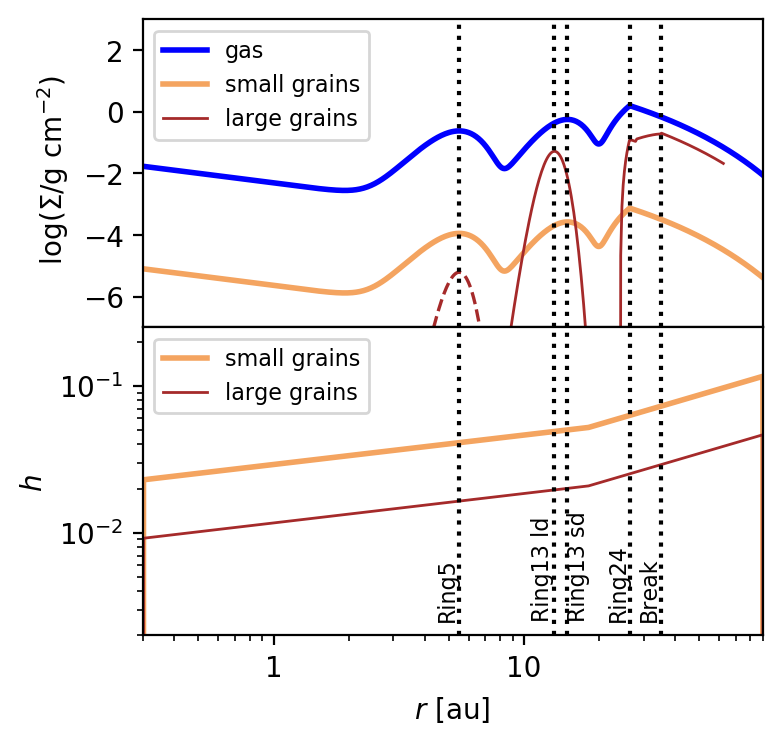
\includegraphics[width=\columnwidth]{allprofiles.png}
    \caption{Top panel shows the surface density profiles for the gas, the large and small grain populations. Bottom panel shows the scale height $h(r)$ as a function of polar radius. The dashed lines crossing both panels are the radii that confine the structures.}
    \label{fig:profiles}
\end{figure}

The final structure of the parametric model goes as Fig. \ref{fig:profiles} shows. The inner radius of the model grid was set to 0.1\,au and an otter radius of 115\,au, large enough for the dust disc to become undetectable.

The dust begins at 0.3\,au, out of the zone expected to be cleared by dynamical interactions with the central binary \citep{Art_Lu}. For the small dust grains, we propose a three ringed structure. The innermost ring of the model is located from 5 to 8\,au ,this ring is not present in the observations but was added for having a better SED fit. Then follows the two observed rings: the first goes from 12 to 19.5\,au and, with a 1\,au-wide gap between them, the outer ring goes from 20.5\,au and has its maximum density peak at 25\,au. The small-dust density then then fades as the radius increases.

On the other hand, in order to reproduce the two ringed observed morphology of the millimetre continuum emission we required a model that has its large-dust grain population distributed with a wide central cavity (r = 12.3\,au), a narrow 2.6\,au-wide inner ring followed by a gap of 8.2\,au that separates both rings and then an outer ring that goes from 23\,au and has it density peak at 27.3\,au. This last ring has a break between 32 and 34.5\,au and then reaches out to 57\,au.

For the vertical structure, \citet{dOrazi} found flaring angles of $\varphi$ = 6.2$\pm$0.6\,$\degr$ for the inner ring and $\varphi$ = 8.5$\pm$1.0\,$\degr$ for the outer one. For that matter, the model uses two different flaring index $\psi$. The separation between the two values was set at $r$ = 19\,au with values of 0.2 and 0.5 for the inner part and the outer part respectively. Also, the scale height is calculated using $H_o$ = 0.045 and $r_0$ = 19.5\,au.

We set the values of the inclination an the position angle as the same as those obtained from the ALMA observation in Section \ref{sec:Observations}, so the model has an inclination of i = 33.9\,$\degr$ and a P.A. = 74.6\,$\degr$. Finally, the distance is set at d = 72.4\,pc \citep{Gaia}.

\section{Model results and discussion} \label{sec:results}

Our parametric model is fairly successful in reproducing the available data. The simulated images and the SED of the model are shown in Fig. \ref{fig:two} and Fig. \ref{fig:SED} respectively.

The simulated image at 1.65\,$\micron$ shows a similar radial structure to the one visible in the observations, displaying a two ringed disc, where the innermost small-dust ring of the parametric model hides under the artificial coronagraph. The visible asymmetry in the SPHERE observations is recreated using grains larger than 0.4\,$\micron$ as smaller grains do not cause a strong forward scattering, meaning that the disc is depleted of very-small grains. Interestingly, the model accurately shows the shadows described by \citet{dOrazi} that are present in the SPHERE-IRDIS image.

The simulated 1.3\,mm continuum image displays some clear similarities with the ALMA observation. The model reproduced the two rings that are present in the observation: the faint inner ring and the outer brighter one. As the radial profiles obtained from the simulated images of the model closely resemble those deduced from the observations (Fig. \ref{fig:radprofiles}), we can assume that the model provides a reliable approximation of the disc structure, including, particularly for our interest, the dimensions of the previously unseen 1.3\,mm thin inner ring. Accordingly, taking the parametric model values for the large-dust inner ring we have that it is located at 13.6\,au, has an estimated width of 2.6\,au, an estimated scale height ranging from 0.25 to 0.32\,au and a dust mass of about 3\,M$_{\earth}$. For the outer ring, we have that it has an intensity peak at $\sim$30\,au, a break present at $\sim$35\,au and a mass of $\sim$43\,M$_{\earth}$

As \citet{2018ApJ...869L..46D} explains, the stability of a narrow dust ring can be analysed comparing its height to its radial extent. For a ring to be stable and long-lived its horizontal dimension can not be less than its vertical height. Using the parametric model scale height of 0.28\,au at 13.46\,au and the measured width of the inner ring (4.17\,au, see Section \ref{sec:Observations}), we have that its width is $\sim$15 times its scale height, meaning that it is stable.

Fig. \ref{fig:SED} shows the SED constructed from the model compared to the photometry data available in the literature in \citet{Jensen_97} and online in \textsc{vizier} and \textsc{diana}, and also using spectrometry data from an archival \textit{Spitzer} IRS spectrum. From the similarity between the data and the resulting SED of the model we confirm that there has to be a small-grain population close to the stars down to 0.3\,au. The decision of employing the three ringed structure for the small dust grains relies on the fact that the SED needed a ring at a radius smaller than 10\,au to have a proper fit, this proposed ring has not been observed. The unexpected central emission in the 1.3\,mm continuum image could be part of this inner ring and, as it is asymmetric, the ring could be lopsided.

\begin{figure}
	\centering
	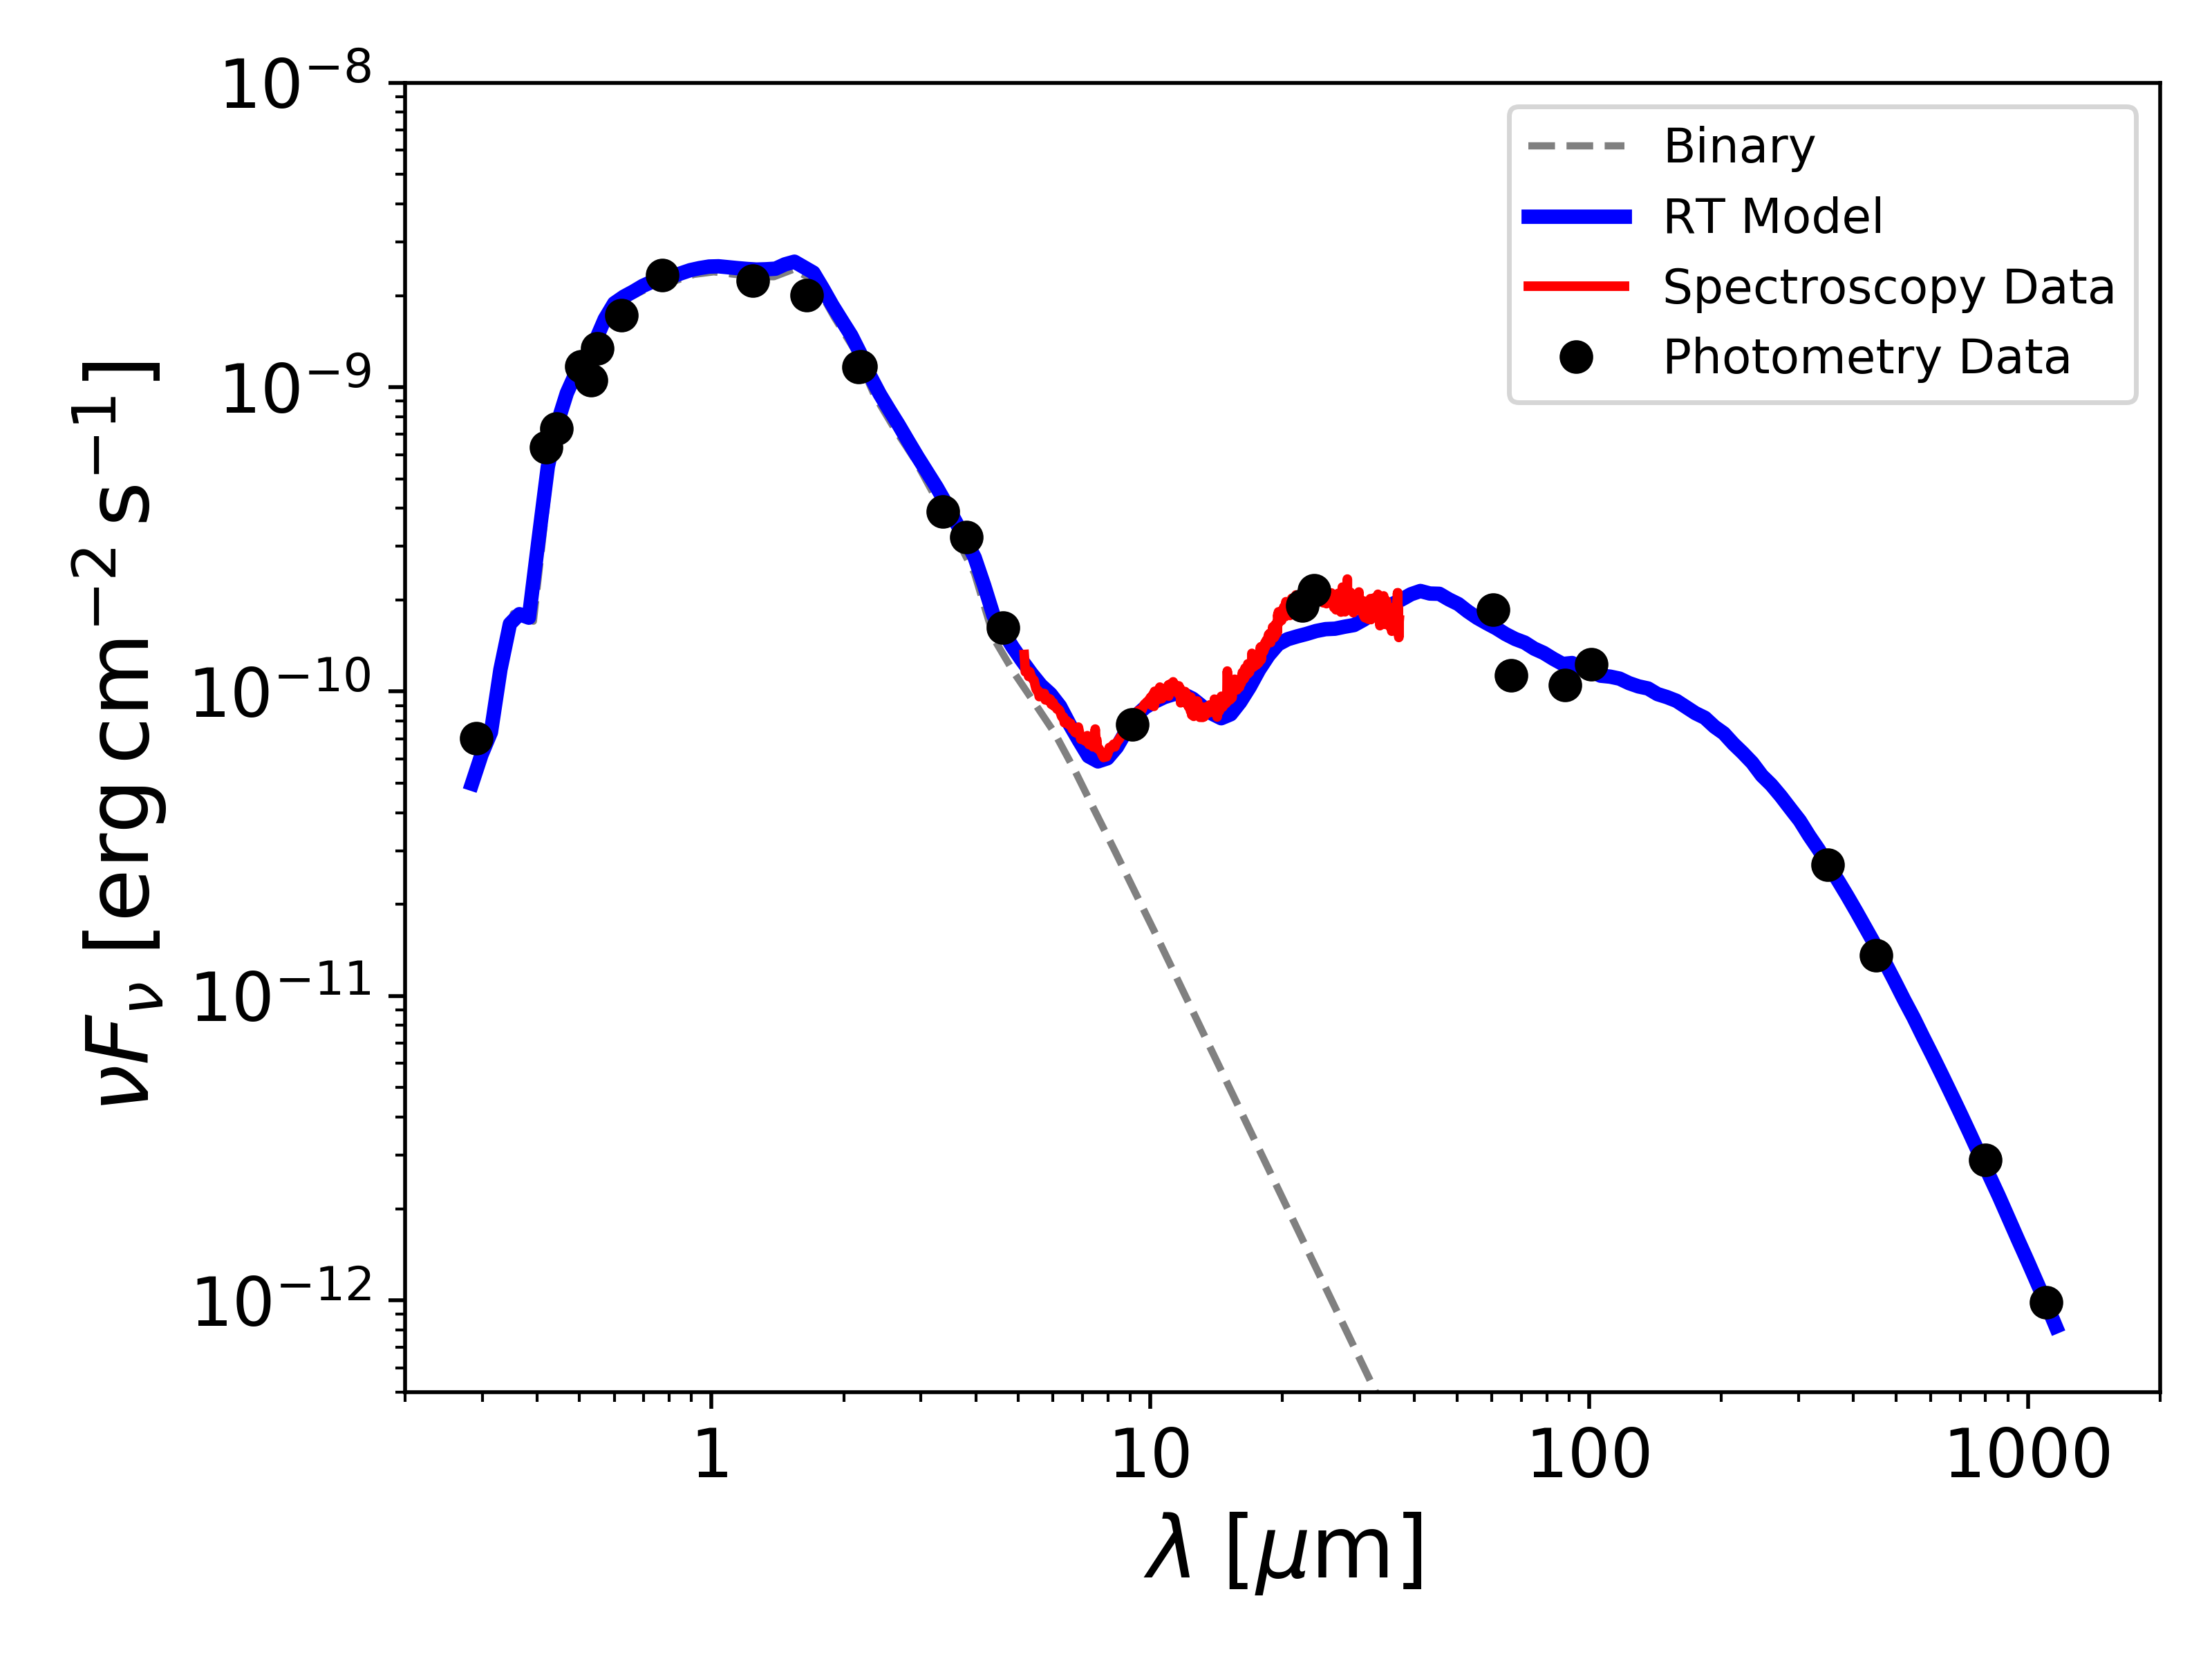
\includegraphics[width=\columnwidth]{SED_.png}
    \caption{The SED (black points and solid red curve) compared with the model (blue). The black points represent the measured photometry and the red line shows an archival \textit{Spitzer} IRS spectrum. The dashed silver curve shows the emission of the stellar photosphere model.}
    \label{fig:SED}
\end{figure}


%\begin{table}
% \caption{Model rings masses}
% \label{tab:masses}
% \begin{tabular}{lcc}
%  \hline
%  Ring & Location & Mass\\
%   & $\mathrm{au}$ & $M_{\earth}$ \\
%  \hline
%  First & 5 to 8 & 0.0007 \\
%  Second & 11 to 19 & 2.9 \\
%  Third & 20 to 80 & 43 \\
%  \hline
% \end{tabular}
%\end{table}


\section{Conclusions} \label{sec:Conclusions}

New ALMA 1.3\,mm continuum imaging of the circumbinary disc around V4046\,Sgr reveals new information about its substructure. Using a radiative transfer model and decompositions in polar coordinates of the computed \textsc{uvmem} model image, we measured and analysed the previously unseen thin inner ring and studied the small-dust population distribution.

The key conclusions of our analysis are as follows.
\begin{enumerate}

  \item We report a narrow inner ring for the 1.3\,mm continuum located at 13.46$\pm$0.43\,au from the stars and has an estimated width of 4.17$\pm$0.94\,au. The location of this ring is similar to the inner ring observed in the scattered-light image, revealing that the ring includes a considerable mass of millimetre-sized grains of around 3\,M$_{\earth}$. Using the parametric model scale height value ($h= $ 0.28\,au at 13.46\,au) we have that the ring width is $\sim$15 times its estimated height, making it a stable ring.
  
  \item The 1.3\,mm outer ring, that starts at $\sim$23\,au and has its peak intensity at $\sim$32\,au, presents a visible break in the surface brightness at $\sim$35\,au. 
  
%\item The inner ring may not be totally resolved as its width is comparable to the beam size. Future observation with smaller beams sizes could give an answer on the real radial extent of the ring.
  
  \item We interpret the asymmetry observed with SPHERE-IRDIS at 1.65\,$\micron$ as due to strong forward-scattering, which implies that the dust population is depleted of grains smaller than $\sim$0.4\,$\micron$.
  
  \item As our parametric model accounts for the SED of the system, the disc requires the existence of a sub-micron dust population close (<5\,au) to the stars. We also predict the existence of another thin ring at $\sim$6\,au, about 3\,au-wide and made of small dust grains that lies under the coronagraph of the scattered-light image. Additionally, the weak central emission at 1.3\,mm could be part of this ring.
\end{enumerate}
  
Finally, we encourage additional detailed analysis and more modelling that could give some explanations of the substructures present on the disc. Higher resolution observations of radio continuum may provide the opportunity to make better measurements of the rings radial extension. For future radiative transfer models, it might be worth adding gas, using different inclinations for the inner and outer disc and implementing hydrodynamic simulations too, especially to try to unravel the mystery of how the inner ring is so thin an stable. 

\section*{Acknowledgements}

Try to keep it short.

\section*{Data Availability}

%%%%%%%%%%%%%%%%%%%% REFERENCES %%%%%%%%%%%%%%%%%%

% The best way to enter references is to use BibTeX:

\bibliographystyle{mnras}
\bibliography{bibtex} % if your bibtex file is called example.bib


% Alternatively you could enter them by hand, like this:
% This method is tedious and prone to error if you have lots of references
%\begin{thebibliography}{99}
%\bibitem[\protect\citeauthoryear{Author}{2012}]{Author2012}
%Author A.~N., 2013, Journal of Improbable Astronomy, 1, 1
%\bibitem[\protect\citeauthoryear{Others}{2013}]{Others2013}
%Others S., 2012, Journal of Interesting Stuff, 17, 198
%\end{thebibliography}

%%%%%%%%%%%%%%%%%%%%%%%%%%%%%%%%%%%%%%%%%%%%%%%%%%

%%%%%%%%%%%%%%%%% APPENDICES %%%%%%%%%%%%%%%%%%%%%

%%%%%%%%%%%%%%%%%%%%%%%%%%%%%%%%%%%%%%%%%%%%%%%%%%


% Don't change these lines
\bsp	% typesetting comment
\label{lastpage}
\end{document}

% End of mnras_template.tex
